\section{Introduction}
% Just a first sketch:
This Bachelor Thesis is about writing a fast and interactive visualization environment suitable for scientific computing. 
As GUI elements and editable text fields are supplied, one can also write and execute scripts, and immediately visualize all bound variables of the script and edit them via simple GUI elements like sliders. The focus is on creating a modular library, that is written in a fast high-level language, making the library easy to extend.
The introduction is structured in the following way.
First, an introduction to the general field of research and its challenges is given. 
From these challenges, the problems relevant to this thesis will be extracted.
Finally this chapter will conclude with a solution to the problem, how to measure the success and give an outlook on the structure of the entire Bachelor Thesis.
 
\subsection{Field of Research and Problem}


%Scientific computing: visual debugging, interactive programming, high performance
%First rough sketch:
It's not immediately visible, but the very general research field is making computer science more accessible and understandable. 
Visualization and interaction do make opaque processes more accessible, by giving the user the ability to look at data and algorithms from different perspectives. 
One example can be this function f(x,y,z)=sin(x/15)+sin(y/15)+sin(z/15), which describes a 3D volume. 
This is a simple function, which is already not that easy to interpret. In figure \ref{fig:volume}, you can see different visualizations of f. Especially for more complex functions, visualizing might be the only way to get a deeper understanding of the values that an algorithm produces.
It is also very helpful to debug the actual math and not just the program. For example by visualizing the rotation from a rotation matrix, immediately makes it visible if the wanted effect was achieved.
This is especially relevant for users, who don't have a broad background in computer science, or programmers implementing complicated state of the art algorithms.
These users can be found especially in scientific computing, which is why this thesis focuses on scientific computing. 

More precisely, it focuses on research which involves writing short scripts, while visualizing the results is helpful. 
An example would be a material researcher, who is investigating different 3D shapes and materials and their reaction to pressure.
The researcher would need to read in the 3D object he wants to analyze, have an easy way to tweak the material parameters and it would be preferable to get instant feedback on how the pressure waves propagate through the object.

Several demands by the researcher makes it challenging to offer software for this area.
Lets look at one of the challenges at a time:

\begin{itemize} 

    \item  \textbf{Visualizations}

    Visualizations are a key element to the understanding and access of complicated algorithms.
    In some domains, problems become only manageable by visualizing them.
    The problem with that is, that a visualization which successfully captures the gist of the data is pretty hard.
    To leverage this problem, the visualization API should be intuitive to use and very flexible, to allow the researcher to build highly customized visualizations for his problem.
    Also, research is getting published, together with visualizations explaining the results. As they represent the research to the public, they should be as understandable as possible and preferably look good.
    Offering a creative, interactive work flow can make this challenge considerably easier.

    \item \textbf{Money and Time is constrained}
    
    This means the research has to conclude quickly and most likely, it is not an option to employ a person or even a company to solve sub problems.
    From this we can deduce three preferences: 
    The used libraries should be accessible to the researcher, because when something doesn't fit his demands, he most likely needs to resolve it himself due to constrained resources.
    If code needs to be written to solve this, it should be in an easy to understand high-level language, otherwise the sub problem can considerably slow down the research.

    \item \textbf{Speed}
    
    Speed can be both seen as a usability or a time/money constraint. 
    Time and money constraints become clear, if the computation times are very big. If one library is 60 times slower than the other, it might not matter if the task only takes \SI{d-5}{\second}. But it does matter if the fast computation takes a day, leaving the slow library with a computation time of 60 days.
    This would mean for researchers, that they either have to buy more powerful computers, or deal with the lost time.
    But also for small numbers in the second range, a difference of 20 times slower can have a big impact on the researchers productivity. If the computation is repetitive, like trying out all the different materials, this has an immediate influence on how many material combinations the researcher can try out in one day.
    More subtle is the influence of speed on a simple task like changing the color. If the color slider stutters, it is completely possible to change the color, but it will be a frustrating user experience. 
    This is why the whole system should be designed to offer top notch speed, to not run into these kind of issues.

\end{itemize} 


\subsection{Problem Solutions and Measurements of Success}
%* Write it in one, open source, high level, high performance language (Julia)
%* Write it in OpenGL
%* Open Source
%* Easy ways of creating GUIs
%* Modularity
%* Offer a broad variety of visualization

\subsubsection{Visualizations and Interaction}

Having visualizations are the main purpose of the written software in this thesis.
% Measurements


\subsubsection{Extensibility}
As previously deduced, extensibility is an important factor, which can decide, if a library is fit for scientific computing or not. 
It's not only that, but also a great factor determining growth of a software, as the more extensible the software is, the higher the probability that someone else contributes to it.
In order to write extensible software, we first have to clarify what extensibility is.
Extensible foremost needs, that the code is accessible. There are different levels of accessibility. The lowest level is closed source, where people purposely make the code inaccessible. While this is obvious, this is just a special case of not understanding the underlying language. Just shipping binaries without open sourcing the code, means that the source is only accessible in a language which is extremely hard to understand, namely the machine code of the binary. So other examples for inaccessibility are writing in a language that is difficult to understand. Other barriers are obfuscated language constructs, missing documentations and cryptic highly optimized code.
Further more the design of the library in the whole is an important factor for extensibility. It's not only important, that all parts are understandable, but also, that every independent unit in the code solves only one problem. 
If this is guaranteed, re-usability in different contexts becomes much more simple. This allows for a broader user base, which in turn results in higher contributions and bug reports. 
Short concise code is also important, as it will take considerably less time to rewrite something, as the amount of code that has to be moved is shorter and less time is spend on understanding the code.

So the code written for this thesis should be open source, modular, written in a high level language and concise.


\vspace{1em}
\begin{minipage}{\linewidth}
    \centering
    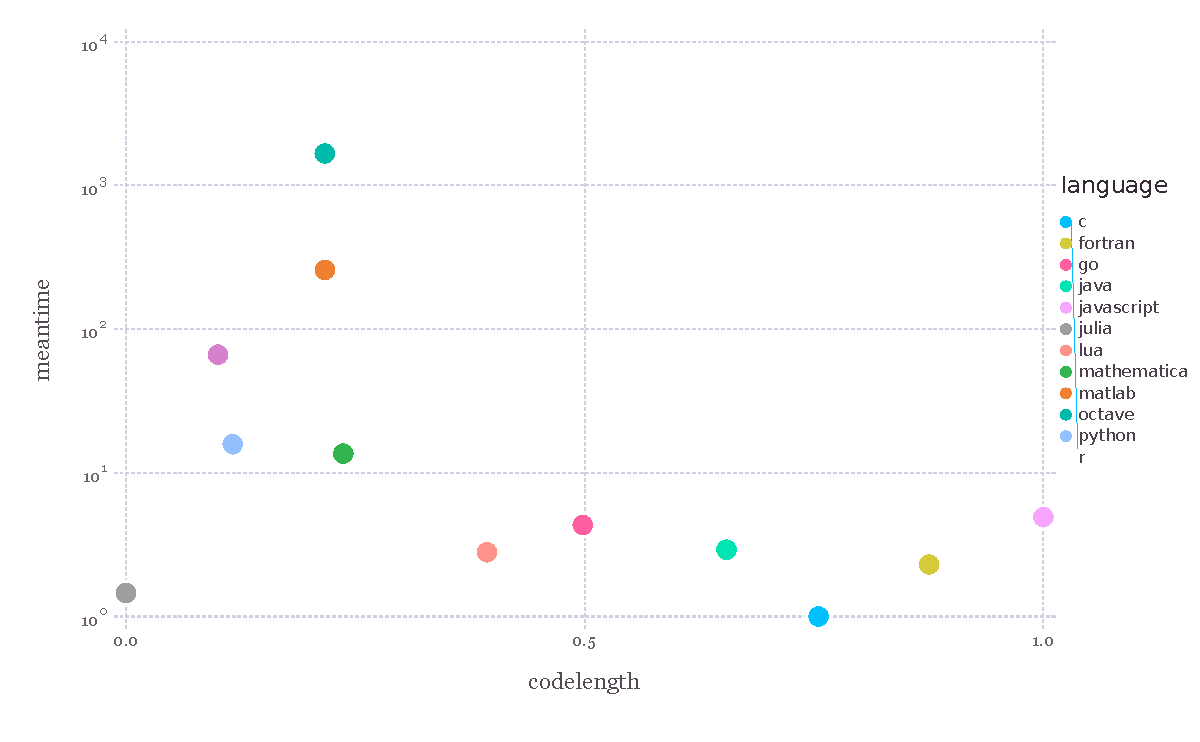
\includegraphics[width=0.9\linewidth]{graphics/julia_bench.pdf}
    \captionof{figure}[Volume Visualization]{Languages speed relative to C (averaged benchmark results), plotted against the length of the needed code}
    \label{fig:juliabench}
\end{minipage}

\subsubsection{Speed}

How to achieve state of the art speed with a high level language is an on going research and basically the holy grail of language design.
Luckily, there is Julia building upon \ac{LLVM}, promising a concise, high-level programming style, while approaching C-performance. 
This is well illustrated in figure \ref{fig:juliabench}.
\ac{LLVM} is a nice compiler infrastructure, which has frontents for different languages and back-ends for different chip architectures. 
A language designer has the task, to emit \ac{LLVM} \ac{IR}, which than gets just in time compiled and optimized to the architecture by \ac{LLVM}.
This concept is very nice, as you can accumulate state of the art optimizations in one place, making them accessible to many languages, while being able to compile to different platforms. There are x86, ARM, OpenCL and CUDA backends. While Julia doesn't support them all, it will hopefully be possible in the future. 
\ac{LLVM} is also used by Clang, the C/C++ frontend for \ac{LLVM} rivaling gcc and for Apple's programming language Swift. 
This makes \ac{LLVM} is a very solid basis for a programming language, as these are highly successful projects giving  \ac{LLVM} a lot of drive(source!?).
See table \ref{table:FEComparison}, for a little benchmark.

To get high performant 3D graphics rendering, there are on the first sight a lot of options.
If you start to take the previously demands into account, the options shrink down.
It should be implemented in one high level language, which can be used for scientific computing and has state of the art speed. At this point, there are close to zero libraries left. As you can see in figure \ref{fig:juliabench}, Matlab, Python and R disqualify, as they are too slow. JavaScript, Java, Go and Lua are missing a scientific background and the others are too low level for the described goals.
This leaves only Julia, but in Julia there weren't any 3D libraries available, which means that one has to start from scratch.
There are only a couple of GPU accelerated low-level libraries available, namely OpenGL, DirectX and Mantel, which are relatively comparable. This leaves one library, if you additionally introduce the constraint of cross-platform compatibility.
So for the purpose of high speed visualizations, OpenGL was wrapped with a high-level interface written in Julia. This leaves us with one binary dependency not written in Julia, namely the video driver, which implements OpenGL.

\subsection{Outlook}
%Structure of BA and a few worts on the results 

\subsection{Used Technologies}

\subsubsection{Julia}
\subsubsection{OpenGL}


\subsection{Similar Work}

\subsubsection{Other Languages}
\subsubsection{Ipython Notebook}
\subsubsection{Matlab}
\subsubsection{Mathematica}
\subsubsection{Other Graphic acceleration APIs}